\chapter{Einleitung}
\section{Abgrenzung des Themas}
	Cognito ergo sum blabla...
	\todo{Definitionen bla und blabla ausschließen}
	
	Ein \ac{AST} kann zu weiteren \acp{AST} transformiert werden, auch wenn dies keinerlei Sinn und Zweck ergibt.  \cite[vgl.~S.~255]{Osmani2012}
	
	Die \gls{Same-Origin-Policy} gilt für Ressourcen mit einem Speicherverbrauch $\leq \SI{0}{\byte}$ oder $\geq$ $\SI{1,4}{\mega\byte}$ und für alle anderen Ressourcen.
	
	
\section{Abbildung}
	\begin{figure}[H]\centering
		\begin{subfigure}{.781\textwidth}
			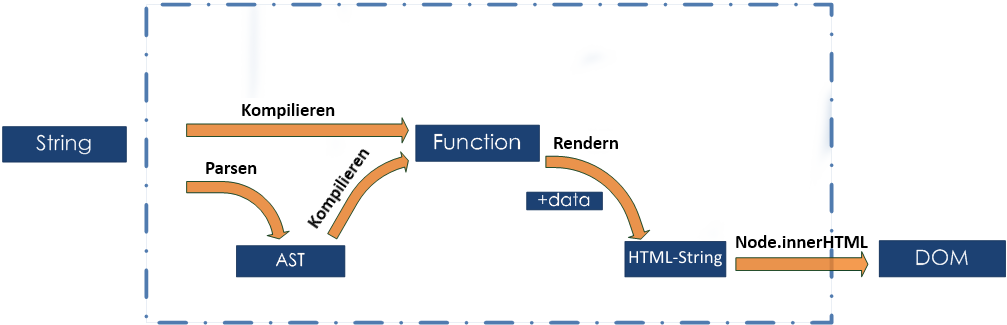
\includegraphics[height=.16\textheight]{./include/abbildungen/String-based-Template}
			\caption[String-basiertes Templating]{String-basiertes Templating\textsuperscript{*}}
			\label{fig:String-based-Template}
		\end{subfigure}
		
		\begin{subfigure}{.781\textwidth}
			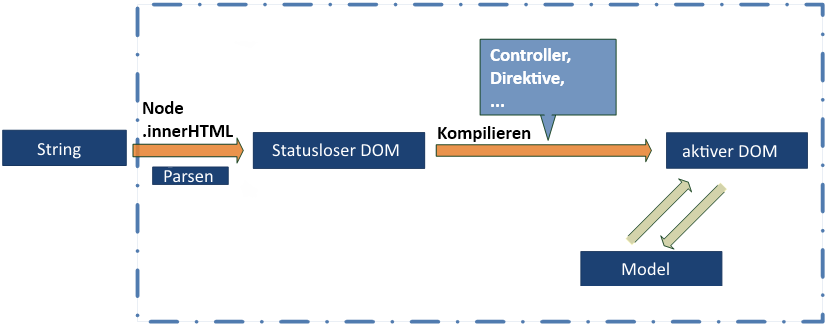
\includegraphics[height=.16\textheight]{./include/abbildungen/Dom-based-Template}
			\caption[Dom-basiertes Templating]{DOM-basiertes Templating\textsuperscript{*}}
			\label{fig:Dom-based-Template}
		\end{subfigure}%
		\label{fig:templatingKonzepte}
		\caption{Templating Konzepte im Vergleich}
		{\scriptsize\textsuperscript{*}Veröffentlichung unter \href{https://github.com/regularjs/regular/blob/master/LICENSE}{MIT License} \cite[vgl.~Abbildungen des Artikel]{RegularJS2015}}
	\end{figure}

	\cref{fig:String-based-Template} zeigt etwas ganz Anderes als das \cref{lst:backboneExtend}.
	\begin{figure}[h]
		\begin{lstlisting}
var Person = Backbone.Model.extend({        //Person erbt von Model
	name: "", age: 0,
	initialize: function(){                       //Constructor-Funktion
		this.on("change:name", function(model){ 
			console.log("Name: " + model.get("name")); 
		}
	}
}),
var student = Person.extend({ matrNr : 0 });//Student erbt von Person
var p1 = new Person({ name: "p1", age: 18 }),
student = new Student({ name: "s1", age: 20, matrNr: 139 });
\end{lstlisting}
		\captionof{lstlisting}{Auswahlbox AngularJS Template}
		\label{lst:backboneExtend}
	\end{figure}
\section{Tabellen}
	Tabellen gibt es hier unter \cref{tab:LinesOfCode} und \cref{tab:NetzwAnalyse}
	\begin{table}[htbp] 
		\as{1.2}
		\scriptsize
		\begin{tabular}{@{}lSSR@{}}
\toprule
		& \text{AngularUI} & \text{DevExtreme} & \\
\midrule
	Datagrid		&	110	&	 40 & \SI{-63,6}{\percent} \\
\midrule[.2pt]
	Controller		&	250	&  	190 & \\
	Service			&	 45	&  	140 & \\
	\emph{Gesamt}	&  	295	&   330 & \SI{11,9}{\percent} \\
\bottomrule
\end{tabular} 
\caption{Anzahl Codezeilen Implementierungen mit DevExtreme im Vergleich zu AngularUI}
		\label{tab:LinesOfCode}
	\end{table}
	\begin{table}[htbp] 
		\as{1.2}
		\scriptsize
		\begin{threeparttable}
\newcommand{\hdrAnfragen}{\textbf{n}\tnote{a}}
\newcommand{\hdrDatenmenge}{\textbf{kB}\tnote{b}}
\newcommand{\hdrDauer}{\textbf{ms}\tnote{c}}
\begin{tabularx}{\linewidth}{@{}Xlcrrcrrcrr@{}}
\toprule
	\multicolumn{1}{c}{\textbf{Aktion}} & \multicolumn{1}{c}{\textbf{Art der Res-}} & \multicolumn{3}{c}{\textbf{ASP.NET}\tnote{1}} & \multicolumn{3}{c}{\textbf{AngularJs}\tnote{2}} & \multicolumn{3}{c}{\textbf{DevExtreme}\tnote{3}} \\[-2.5pt]
		& \textbf{source} & \hdrAnfragen & \hdrDatenmenge & \hdrDauer & \hdrAnfragen & \hdrDatenmenge & \hdrDauer & \hdrAnfragen & \hdrDatenmenge & \hdrDauer \\
\midrule
	\textbf{Start der Anwendung} & JS & 10    & 423,1 & 933   & 8     & 417,3 & 43    & 9     & 1.510,2 & 374 \\
		& HTML  & 1     & 17,4  & 210   & 3     & 4,9   & 36   & 2     & 7,0   & 14 \\
		& \textbf{JS+HTML} & \textbf{11} & \textbf{440,5} & \textbf{1.143} & \textbf{11} & \textbf{422,2} & \textbf{79} & \textbf{11} & \textbf{1517,2} & \textbf{388} \\
\cdashline{2-11}
		& \textbf{XHR} & \textbf{1} & \textbf{1,0} & \textbf{171} & \textbf{1} & \textbf{0,8} & \textbf{7} & \textbf{1} & \textbf{0,8} & \textbf{7} \\
\midrule[.005em]
	\textbf{Marke: VW} & \textbf{XHR} & \textbf{2} & \textbf{0,8} & \textbf{312} & \textbf{1} & \textbf{2,9} & \textbf{4} & \textbf{1} & \textbf{2,9} & \textbf{6} \\
\midrule[.005em]
	\textbf{Model: Golf} & \textbf{JS} & \textbf{1} & \textbf{3,2} & \textbf{640} &       &       &       &       &       &  \\
\cdashline{2-11}
		& \textbf{XHR} & \textbf{2} & \textbf{4,1} & \textbf{1.086} & \textbf{2} & \textbf{809,2} & \textbf{483} & \textbf{2} & \textbf{809,2} & \textbf{483} \\
\midrule[.005em]
	\textbf{Baujahr: 2012} & \textbf{XHR} & \textbf{2} & \textbf{4,0} & \textbf{883} &       &       &       &       &       &  \\
\cmidrule[.005em]{1-5}
	\textbf{Leistung: 103kW} & \textbf{XHR} & \textbf{2} & \textbf{3,9} & \textbf{691} &       &       &       &       &       &  \\
\cmidrule[.005em]{1-5}
	\textbf{Blättern im Grid} & \textbf{XHR} & \textbf{1} & \textbf{3,4} & \textbf{155} &       &       &       &       &       &  \\
\bottomrule
\end{tabularx}%
\begin{scriptsize}
	\newlength{\tmpSpace}%
	\newcommand{\fixedWidthItem}[3]{%
		\settowidth{\tmpWidth}{#2}%
		\setlength{\tmpSpace}{#3}%
		\addtolength{\tmpSpace}{-\tmpWidth}%
		\item[#1]#2 \hspace*{\tmpSpace}%
	}
	\begin{tablenotes}[para]
		\fixedWidthItem{1}{Original ASP.NET mit DevExpress}{5cm}	\item[a] Anzahl der Anfragen an den Server\\
		\fixedWidthItem{2}{AngularJS mit AngularUI Grid}{5cm}		\item[b] Übertragene Datenmenge in $\SI{}{\kilo\byte}$\\
		\fixedWidthItem{3}{AngularJS mit DevExtreme}{5cm}			\item[c] Zeitdauer der Übertragung in $\SI{}{\milli\second}$
	\end{tablenotes}
\end{scriptsize}
\end{threeparttable}
\caption{Netzwerkanalyse der drei Implementierungen im Vergleich}
		\label{tab:NetzwAnalyse}
	\end{table}
 			
